\section{Materials and Methods}
\subsection{Hypotheses}
\begin{enumerate}
\item Random Forest algorithm has a higher frequency of correctly classifying whales than Random Selection from images
\item Deep Neural Network algorithm has a higher frequency of correctly classifying whales than Random Selection from images
\item Having the knowledge of whales position in a given image increase the frequency of correctly classification of whales with Deep Neural Network
\item Having the knowledge of whales position in a given image increase the frequency of correctly classification of whales with Random Forest
\end{enumerate}


\subsection{Testing Hypotheses}

\subsubsection{Preparation of data}
\begin{figure}
\label{fig:crossvalidation}
\centering
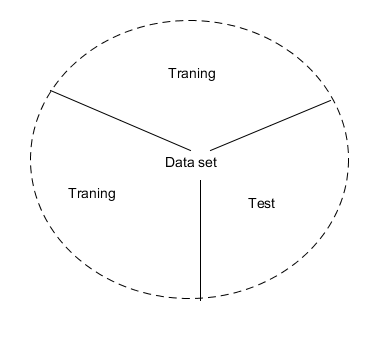
\includegraphics[scale=0.5]{images/3FoldCrossValidation}
\caption{Three fold cross-validation}
\end{figure}

\subsubsection{Testing Hypotheses 1 and 2}

\begin{figure}
\label{fig:testenvironmentraw}
\centering
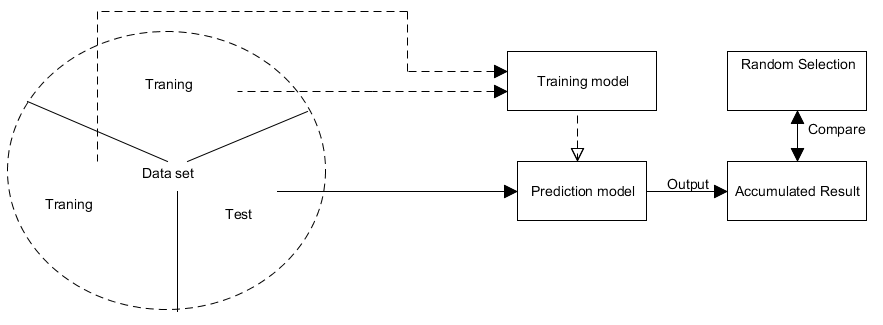
\includegraphics[scale=0.3]{images/EnvironmentOnRawData}
\caption{The testing environment without precessing} 
\end{figure}

\subsubsection{Testing Hypotheses 3 and 4}

\begin{figure}
\label{fig:testenvironmentpre}
\centering
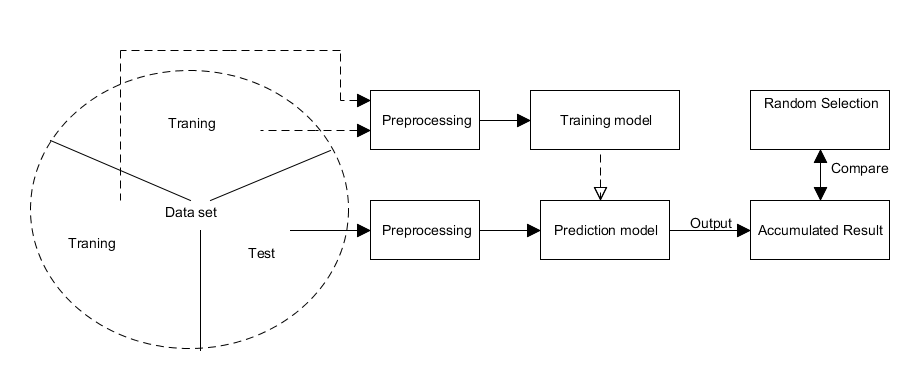
\includegraphics[scale=0.3]{images/EnvironmentWithPre}
\caption{The testing environment with precessing}
\end{figure}
